\documentclass[sigconf,review]{acmart}

\usepackage{subcaption}
\usepackage{cleveref}

\crefname{figure}{Figure}{Figures}

\acmConference[SPLC'25]{29th International Systems and Software Product Line Conference}{September 01--September 05, 2025}{A Coruña, Spain}

\begin{document}

\title{Bridging Digital and Physical: Applying Software Product Line Engineering Principles to Digital LEGO}

\author{Aleksandra Erohina}
\affiliation{
    \institution{FH Upper Austria (FH OÖ)}
    \department{School of Engineering}
    \city{Wels}
    \state{Upper Austria}
    \country{Austria}
}

\author{Christian Zehetner}
\orcid{0000-0002-3149-8476}
\affiliation{
    \institution{FH Upper Austria (FH OÖ)}
    \department{School of Engineering}
    \city{Wels}
    \state{Upper Austria}
    \country{Austria}
}
\email{christian.zehetner@fh-ooe.at}

\author{Georg Hackenberg}
\orcid{0000-0003-3913-4148}
\affiliation{
    \institution{FH Upper Austria (FH OÖ)}
    \department{School of Engineering}
    \city{Wels}
    \state{Upper Austria}
    \country{Austria}
}
\email{georg.hackenberg@fh-ooe.at}

\begin{abstract}
    In this paper, we explore the application of software product line engineering (SPLE) principles to the development of physical products, specifically using digital LEGO as a case study. 
    By translating key concepts from the SPLE community, we demonstrate how modularity, variability management, and systematic reuse can enhance the design and production of physical products. 
    Our experience highlights the benefits and challenges of this interdisciplinary approach, providing valuable insights for both software engineers and product designers.
\end{abstract}

\keywords{Software Product Line Engineering (SPLE); Digital LEGO; Modularity; Variability Management; Systematic Reuse; Physical Product Design; Interdisciplinary Approach}

\maketitle

\section{Introduction}
\label{sec:introduction}

With today's shift from a seller's to a buyer's market, there is a clear trend towards product customization. 
Customers are constantly seeking products that cater to their specific needs and budgets. 
However, creating customer-specific designs can often be inefficient and costly, making it unaffordable for the average consumer.
Besides, in most industries very few or practically no systems are created “from scratch”, so engineers are likely to reuse knowledge from a previous project or product in the form of documents, processes, or models~\cite{Góngora_2015}. 

To find a balance between reuse and customization in software and systems development, software product line engineering (SPLE) has emerged as a viable solution. 
SPLE is an approach to cost-efficiently deriving tailored products for markets and customers, utilizing common components and services in a planned manner~\cite{Runeson_2012}.
The focus is shifted from building isolated products to building families of related products, while reuse is discussed not at an individual object level, e.g.~libraries or components, but as a whole: organizational, process-wise, and also lifecycle-wise end-to-end from requirements to actually deployed variability at the customer~\cite{Schwanninger_2009}. 
This approach involves the development of a core platform as well as reusable components that can be easily customized to meet the specific needs of different products within a product line. 

For example, software products that are being developed for the international market must be adapted for different legal or cultural environments, as well as for different languages, and so must provide adapted user interfaces~\cite{Beuche_2007}. 
To increase software reuse and streamline development processes, developers create a modular software framework that includes common functionalities. 
The framework modules then can be reused across different product models and customized as needed to meet specific requirements for each individual market and customer.

Originating in software development, SPLE principles have now spread far beyond the software domain. 
Companies in many other industries, such as automotive, aerospace, and consumer electronics are taking advantage of reusability and variability management while reducing time-to-market, improving efficiency, and increasing customer satisfaction. 
For instance, Lockheed Martin estimates that because of its SPLE-inspired approach it saves over \$47 million a year ~\cite{Gregg_2015}, while Hewlett-Packard reports that it builds products 10 times as complex, with 1/4 of the staff, in 1/3 of the time, and with 1/25 of the bugs of previous products ~\cite{Mebane_2007}.

However, when it comes to incorporating SPLE principles into the creation of technical systems, particularly when creating geometric representations of product lines of mechanical products, this approach has not yet become widely established. 

\paragraph{Research objective}

To overcome the current situation we work on translating established ideas and concepts from the software product line engineering community to the development of physical (and ultimately cyber-physical) products.
Also, we want to help improving and more widely establishing product line engineering education for designers of physical products.

\paragraph{Research question}

To reach our research objective, we tackle the following research questions here:
Can we use digital LEGO for building interesting use cases for product line engineering?
Can we see typical issues in product line engineering such as module (in-)compatibility in such use cases?
Can we use existing digital LEGO tools for building these use cases already today?

\paragraph{Contribution}

To answer these research questions, we first conduct a literature review on product line engineering in the software domain as well as other domains (see Section~\ref{sec:related-work}).
And then, based on the results of our literature review we derive a digital LEGO case study consisting of atomic modules, various configuration options, and a 150\% model (see Section~\ref{sec:case-study}).

\section{Related work}
\label{sec:related-work}

Subsequently, a literature review about PLE in software domain is provided in Section~\ref{sec:ple-software},
and a literature review about PLE in other domains is provided in Section~\ref{sec:ple-other}.

\subsection{PLE in the software domain}
\label{sec:ple-software}

A software product line is a set of systems that share a common, managed set of features satisfying the specific needs of a particular market segment or mission and that are developed from a common set of core assets in a prescribed way ~\cite{Clements_2002}, where
a feature is a characteristic of a member product in a product line that distinguishes it from other member products in the product line ~\cite{ISO/IEC_26550}.
%A concrete product of a product line is called a product variant.
Van der Linden et al. ~\cite{Linden_2007} formulated several principles that are fundamental in PLE. They include, among others, the principle of the two-life-cycle approach, which includes the domain engineering and the application engineering lifecycle, and the principle of variability management.

Domain engineering is a reuse-based approach defining the scope (i.e., domain definition), specifying the structure (i.e., domain architecture), and building the assets (e.g. requirements, designs, software code, documentation) for a class of systems, subsystems, or member products ~\cite{ISO/IEC_26550}. During domain analysis, developers determine the scope of the software product line and identify its common and variable features, which they then document in a variability model. 
A number of techniques have been developed to manage variability.
For the drone use case, we use the orthogonal variability model (OVM), introduced by Pohl et al. ~\cite{Pohl_2005}. It uses variants and variation points to denote variability, and dependencies to define relationships between variants and variation points.

Application engineering is the process of deriving a single variant tailored to the requirements of a specific customer from a product line, based on the results of domain engineering ~\cite{Kästner_2013}. 
However, with the appearance of second-generation PLE, application engineering shrinks to almost nothing; products are produced through the use of high-end industrial strength automation that configures the shared assets appropriately for each product ~\cite{Krueger_2013}.

PLE goes hand in hand with the concept of modularity. While modularity enables the production of multiple end products from a limited number of modules, PLE manages and optimizes a company's product diversity in order to control complexity and to balance out too many versions.
Li et al. ~\cite{Li_2019} explains modularity as a systematic process where a product or system is composed of various modules, and these modules can be combined in different ways which become different products. However, clear rules should be set up to reassure that all subsystems will fit and function together in the final design ~\cite{Baldwin_2003}. The rules are referred among other things to the module interfaces which define how the interacting modules are connected. The effects of a misspecified interface can go beyond
module incompatibility to unexpected product behavior ~\cite{Parslov_2015}. 

\subsection{PLE in other domains}
\label{sec:ple-other}

When it comes to development of physical products, building blocks of a product in the product line, or shared assets, can include, but are not limited to, requirements, design specifications, design models, source code, build files, test plans and test cases, user documentation, repair manuals and installation guides, project budgets, schedules, and work plans, product calibration and configuration files, data models, parts lists, and more ~\cite{Clements_2015}. 
A product variant is instantiated from a common design that represents all the possible combinations of features for all the possible variants. The design is called a 150\% model, or a superset model, because, as Clements ~\cite{Clements_2015} states, it has the content necessary to support any product in the product line. 

It is well-known that due to software intangibility, hardware engineering cannot be compared to software engineering. 
While applying SPLE principles to the development of hardware, it is important to consider its physical nature, especially when it comes to module interfaces. 
Ulrich ~\cite{Ulrich_1995} states, that interfaces may involve geometric connections between two components or may involve non-contact interactions,  
and that a connection provides a constraint condition at the contact point of the mechanical unit to guarantee the required function of the composition of parts. 
By specifying these geometric constraints in computer-aided design (CAD) models, designers can ensure the proper arrangement and compatibility of parts within the product.

Due to the complexity of dealing with physical dimensions and constraints in 3D modeling, it is not yet possible to apply SPLE principles to physical domain.  
Currently, there is no proof of the existence of a 150\% 3D model, and it is not feasible to generate 3D product variants from such a model. 
In the next section, we propose exploring the application of SPLE principles in designing product lines of physical products, particularly focusing on their geometric attributes.

\section{Case study}
\label{sec:case-study}

In this third chapter we introduce the case study, which is prepared for testing the viability of digital LEGO for product line engineering education.
The selected product line includes three first person view (FPV) drone variants: an ultralight drone, a freestyle drone and a long-range drone, which differ primarily in their performance characteristics.
First, we provide an overview of the atomic modules of the product line, from which the individual variants have been assembled in Section~\ref{sec:atomic-modules}.
Then, we explain the configuration options of the drone use case in the form of a feature tree model in Section~\ref{sec:configuration-options}.
And finally, we introduce the 150\% model for the drone use case in Section~\ref{sec:150-model}.

\subsection{Atomic modules}
\label{sec:atomic-modules}

Each drone is made up of four modules, that deliver a certain function. 
Each module has its own variants, which makes it possible to offer a greater variety of products. 

\subsubsection{Propellers}
\label{sec:propellers}

Propellers shown in \cref{fig:propeller} generate thrust by spinning rapidly, allowing a drone to move in all directions. 
A two-blade propeller provides better efficiency and longer flight times, while a triblade propeller offers more stability and maneuverability. 
Smaller propellers provide better agility, while bigger ones provide more thrust and efficiency, allowing the drone fly longer distances. 
However, larger propellers also require more power to spin.

\begin{figure}[htbp]
    \subcaptionbox{Small size\label{fig:propellor-small}}{
        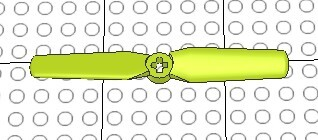
\includegraphics[height=1cm]{./drone-case-modules-propellor-2-small.jpg}
    }
    \hfill
    \subcaptionbox{Medium size\label{fig:propellor-medium}}{
        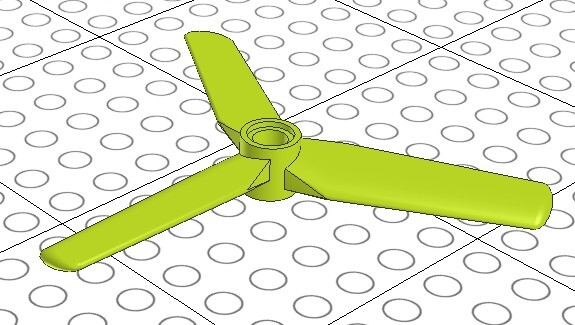
\includegraphics[height=1cm]{./drone-case-modules-propellor-3.jpg}
    }
    \hfill
    \subcaptionbox{Large size\label{fig:propellor-large}}{
        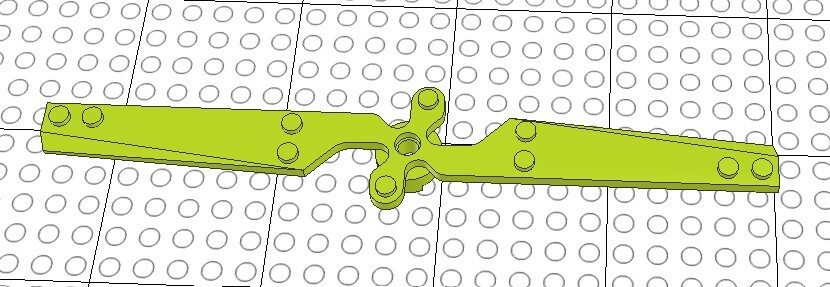
\includegraphics[height=1cm]{./drone-case-modules-propellor-2-large.jpg}
    }
    \caption{Overview of the propeller modules}
    \label{fig:propeller}
\end{figure}

\subsubsection{Batteries}
\label{sec:batteries}

Batteries shown in \cref{fig:batteries} provide power for the drone to operate. 
A smaller capacity battery is lighter and more compact, which can improve the agility and maneuverability of the drone. 
However, smaller batteries have shorter flight times, which means that for longer flights a higher capacity battery is more suitable.

\begin{figure}[htbp]
    \subcaptionbox{Small size\label{fig:battery-small}}{
        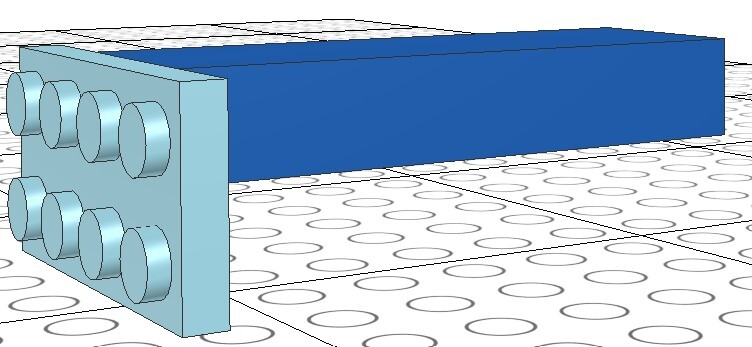
\includegraphics[height=1cm]{./drone-case-modules-battery-small.jpg}
    }
    \hfill
    \subcaptionbox{Medium size\label{fig:battery-medium}}{
        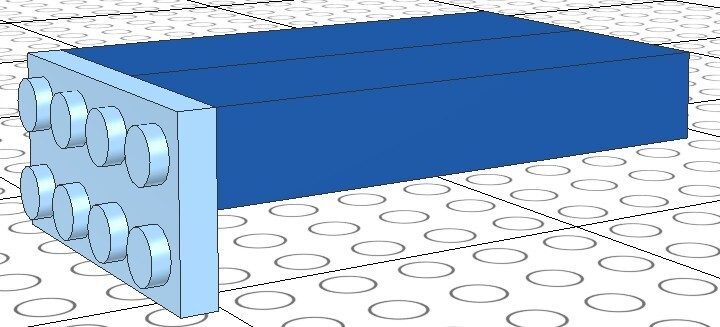
\includegraphics[height=1cm]{./drone-case-modules-battery-medium.jpg}
    }
    \hfill
    \subcaptionbox{Large size\label{fig:battery-large}}{
        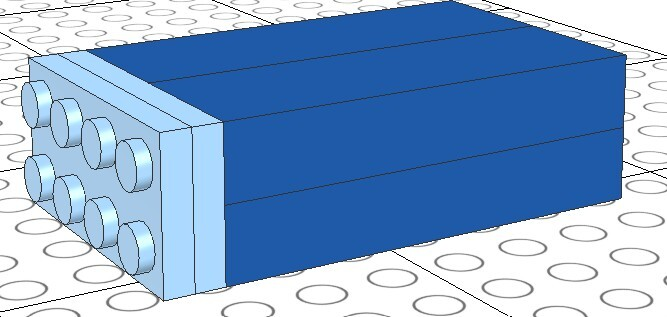
\includegraphics[height=1cm]{./drone-case-modules-battery-large.jpg}
    }
    \caption{Overview of the battery modules}
    \label{fig:batteries}
\end{figure}

\subsubsection{Frames}
\label{sec:frames}

Frames shown in \cref{fig:frames} serve as the structure that holds all the other parts (legs and motors are pre-installed) together. 
A small frame is more maneuverable and agile, while a large frame offers more space for additional components (e.g. larger batteries).

\begin{figure}[htbp]
    \subcaptionbox{Small frame\label{fig:frame-small}}{
        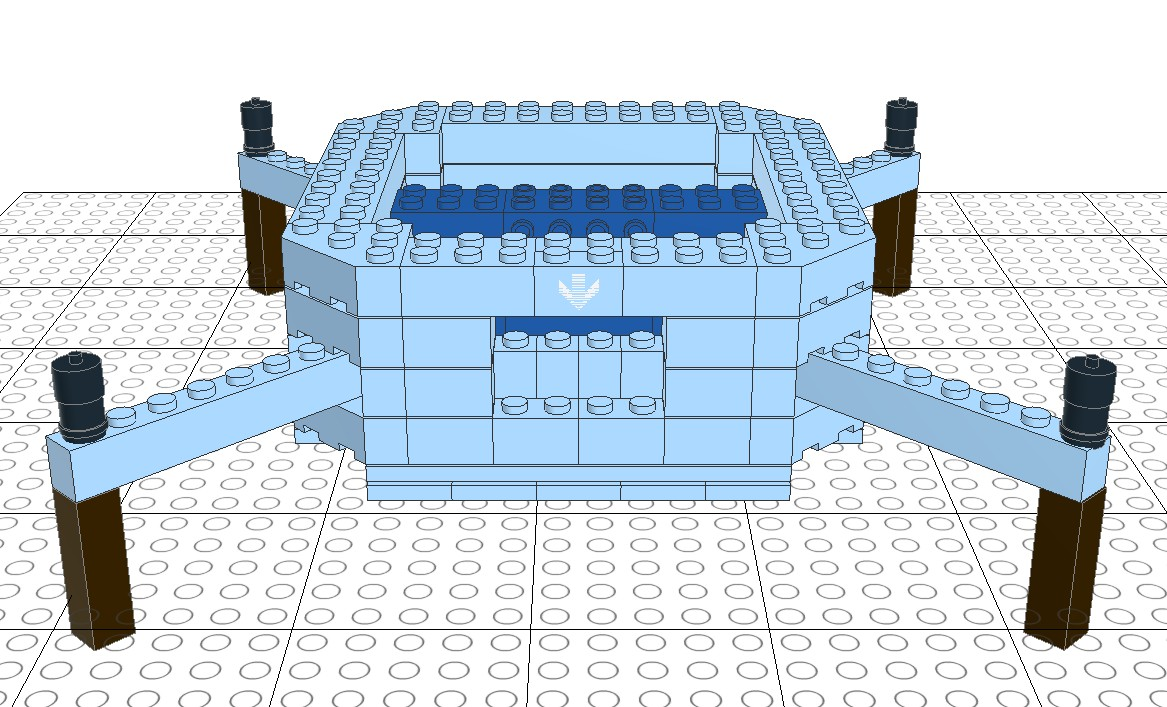
\includegraphics[height=2.1cm]{./SmallFrame.jpg}
    }
    \hfill
    \subcaptionbox{Large frame\label{fig:frame-large}}{
        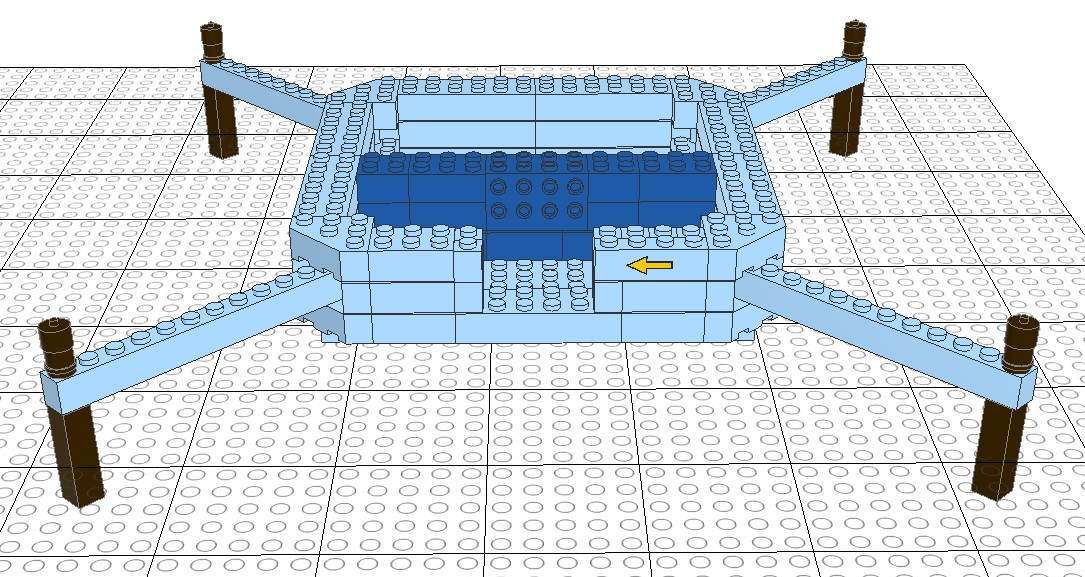
\includegraphics[height=2.1cm]{./LargeFrame.jpg}
    }
    \caption{Overview of the frame modules}
    \label{fig:frames}
\end{figure}

\subsubsection{Covers}
\label{sec:covers}

Covers shown in \cref{fig:atomic-modules} protect internal components of the drone, help to improve aerodynamics and serve an aesthetic purpose as well.

\begin{figure}[htbp]
    \subcaptionbox{Small cover\label{fig:cover-small}}{
        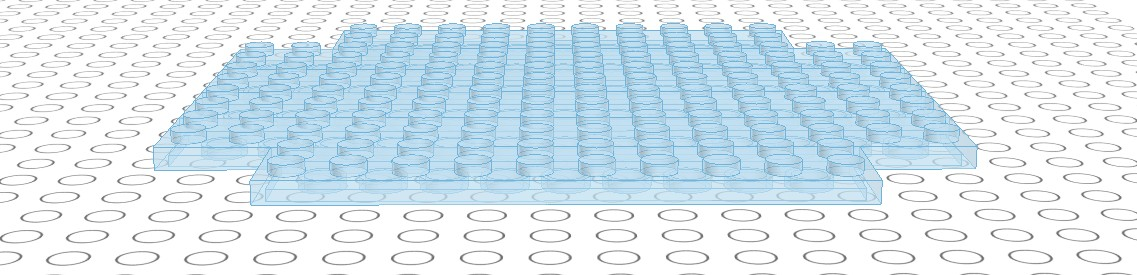
\includegraphics[height=1cm]{./Small Cover2.jpg}
    }
    \hfill
    \subcaptionbox{Large cover\label{fig:cover-large}}{
        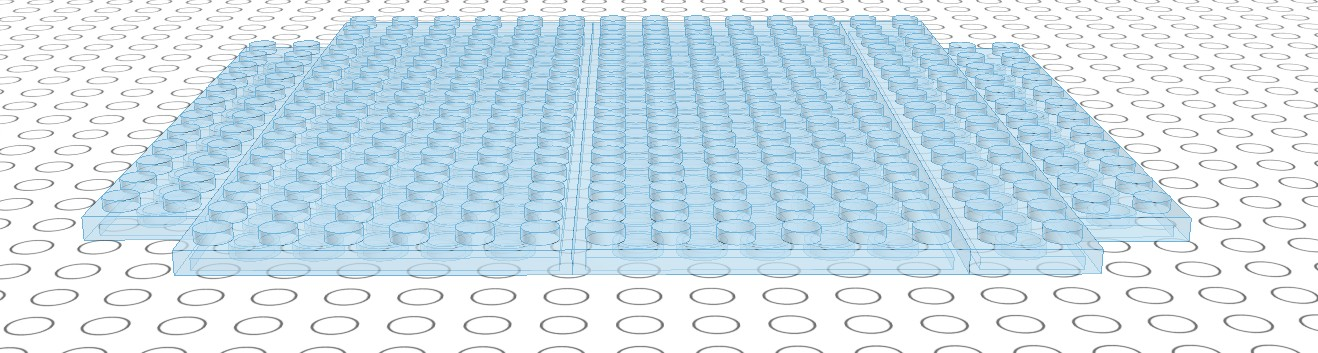
\includegraphics[height=1cm]{./LargeCover2.jpg}
    }
    \caption{Overview of the cover modules}
    \label{fig:atomic-modules}
\end{figure}

\subsection{Configuration options}
\label{sec:configuration-options}

\begin{figure*}[htbp]
    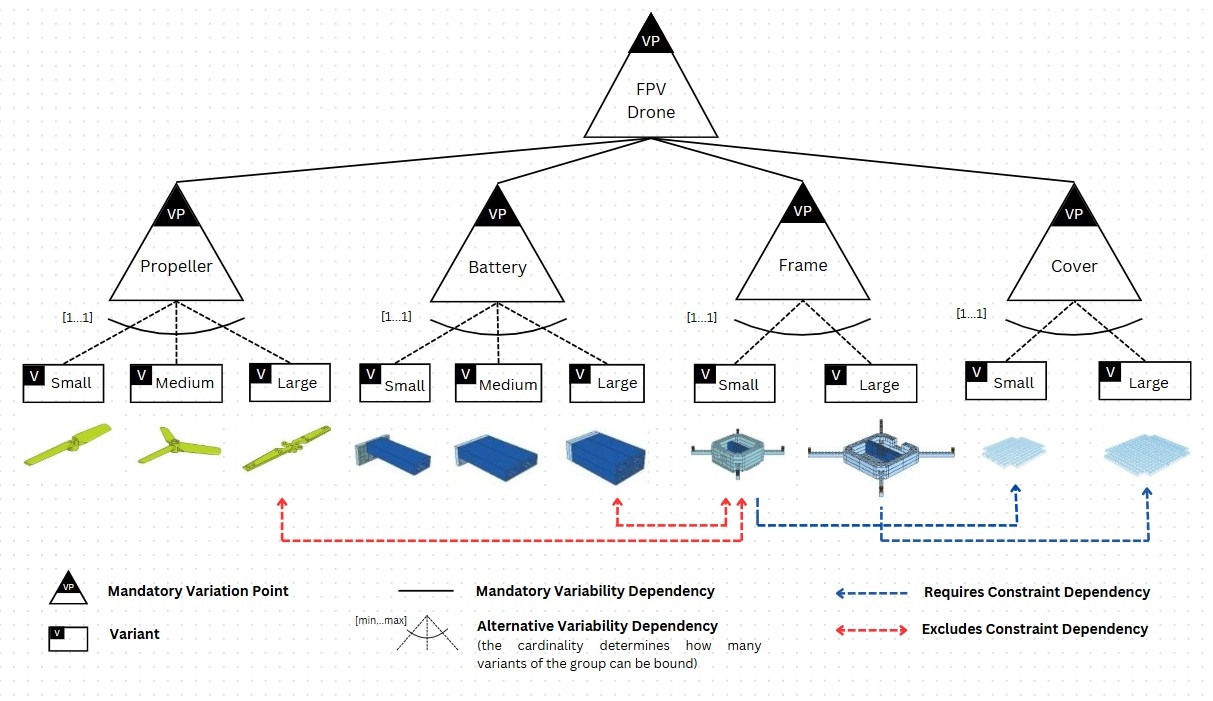
\includegraphics[width=\textwidth]{./FeatureTreeWithLegend3.jpg}
    \caption{Overview of the configuration options for the drone use case}
    \label{fig:feature-tree}
\end{figure*}

The modules can be combined to design customized end products.  
For that purpose, the FPV drone variability model is developed. 
When a customer wishes to design and buy a drone, multiple decisions have to be made before the final system can be build. 
\cref{fig:feature-tree} shows that the variation points Propeller, Battery, Frame and Cover have a mandatory dependency with the FPV drone, which means that they have to be included in the final product. 
For each of these variation points a variant has to be selected. 
The variants are connected by an alternative choice dependency with a minimum and maximum equal to one, which means that only one variant has to be chosen to be included to the final product. 
Additionally, two types of constraint dependencies exist: require constraint and exclude constraint. 
The require constraint means that when the small frame is selected, the small cover should be integrated to the system, and when the large frame is selected, the large cover should be integrated. 
The excluding constraint means that when a large propeller is selected, the small frame can not be integrated to the design and this relationship goes the other way round as well.

\subsection{Interface constraints}

Physical interfaces between interacting modules enable their geometric connection. 
A frame for the drone example has three interfaces: with the batteries, with the propellers and with the covers. 
However, several geometrical constraints should be considered. These include:

\subsubsection*{Size and shape constraints}

Modules must be designed in such a way that they can physically fit together without interference. 
For the drone example, the large frame can accommodate all three types of batteries, while the small frame is limited to only small and medium batteries because of the size constraints.

\subsubsection*{Alignment constraints}

Modules must be aligned properly to ensure proper functioning when assembled together. 
For example, covers must be oriented correctly relative to frames to serve the protective and aesthetic purposes. 

\subsubsection*{Interference constraints}

It is important to consider potential interferences between modules, such as conflicting shapes or components that may impede proper assembly or operation. 
It is technically feasible to install any propeller on any frame, but practical constraints come into play. 
For instance, a large propeller cannot be mounted on a small frame without interference, as it would collide with the frame during rotation.
\cref{fig:feature-tree} illustrates constraint dependencies caused by these geometric restrictions.

\subsection{150\% model}
\label{sec:150-model}

The case study demonstrates the utilization of digital LEGOs to create a 150\% model of a 3D drone architecture. 
The model is built in LeoCAD\footnote{Official LeoCAD website: \url{https://leocad.org}}, which, thanks to its intuitive user interface, is a useful tool for the teaching of various engineering concepts. 
LeoCAD adheres to the LDraw standard\footnote{Official LDraw website: \url{https:/ldraw.org}}. 
\cref{fig:ldraw-standard} demonstrates a meta-model of the LDraw file. The file contains multiple assemblies. 
Each assembly contains multiple references, which point to either a model (which itself can contain sub-assemblies) or bricks (which are standardized and belong to a brick catalog). 
The reference includes transformation data (position, orientation) and optional appearance data (color).

Within the structure of the LDraw file, a main model shown in \cref{fig:150-model} serves as the foundation where all three variants of the drone are instantiated. 
Each variant is further segmented into submodels, which consist of modular components. 
These modules are essentially instances of the submodels, all organized within the same file.
The main model serves as the primary assembly, the three different drone variants are also categorized as assemblies. 
Moreover, components such as modules (e.g., covers, frames, batteries, and propellers) are also classified as assemblies. 
An assembly consists of children, where each child is linked to either a brick or another assembly. 

\begin{figure}[htbp]
    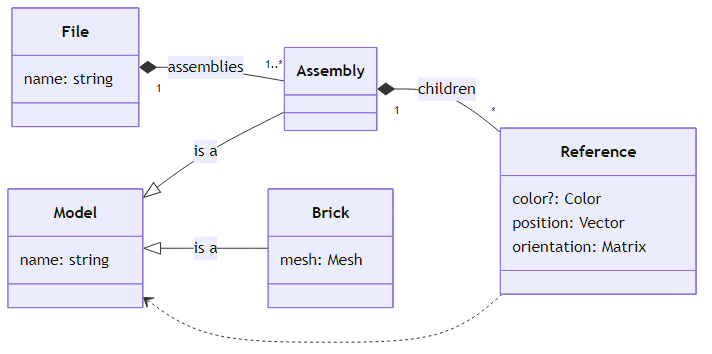
\includegraphics[width=\columnwidth]{./ldraw-standard.png}
    \caption{LDraw standard}
    \label{fig:ldraw-standard}
\end{figure}

The approach enables to reuse the modules and submodels, promoting efficiency and versatility in design. 
The 150\% model encompasses all feasible combinations of drone features across the different variants. 
This abundance of information extends beyond the actual requirements of a specific drone type; for instance, showcasing three distinct battery sizes even though a practical FPV drone would only utilize one.

% \begin{figure}[htbp]
%     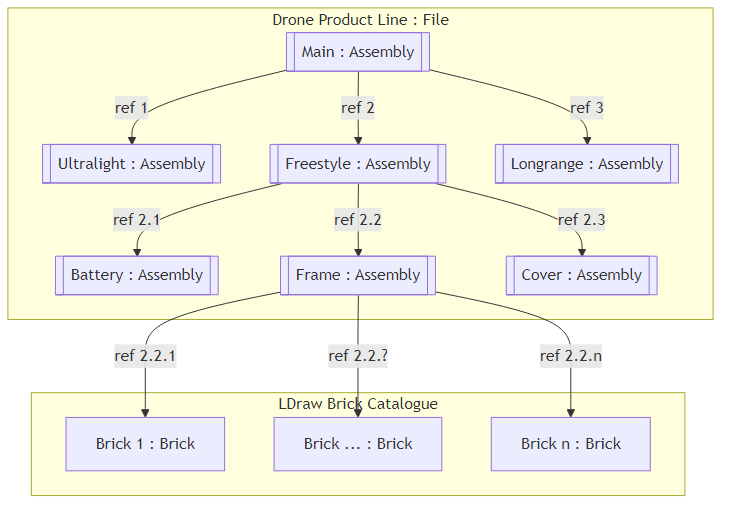
\includegraphics[width=\columnwidth]{./ldraw-model.png}
%     \caption{LDraw model}
%     \label{fig:ldraw-model}
% \end{figure}


\begin{figure*}[htbp]
    \includegraphics[width=\textwidth]{./150_MODEL_6.jpg}
    \caption{Overview of the 150\% model for the drone use case}
    \label{fig:150-model}
\end{figure*}

\section{Conclusion}
\label{sec:conclusion}

The knowledge acquired from the literature review coupled with the case study have provided a comprehensive demonstration of how SPLE principles can be effectively applied to the development of physical products with the usage of digital Lego. 
The first step was to create atomic drone modules, which could then be assembled into individual variants. 
Then, a robust variability model and a comprehensive 150\% model were developed. 
By utilizing these methodologies, we were able to derive a product line comprising three distinct drone variants from the model. 
This allowed us to demonstrate how well digital LEGO is suited to the 150\% modelling and reuse of modules across the entire product line.

In the next steps, we plan to explore geometric interfaces between components of physical products in a product line. Unlike software engineering, the realm of interfacing in this context remains relatively uncharted, making it an interesting area for exploration. 
One aspect to consider is the impact of a change to a single module on the entire product line. 
By examining whether such changes are consistent across all products in the line, we can gain insight into issues related to interface compatibility and mechanical stability. 
The use of digital LEGO is a very promising way to explore this area in an easy way.

\bibliography{main}
\bibliographystyle{ACM-Reference-Format}

\end{document}